\documentclass[border=10pt]{standalone}
\usepackage{tkz-fct}
\usepackage{tkz-base}
\usepackage{array}

\begin{document}

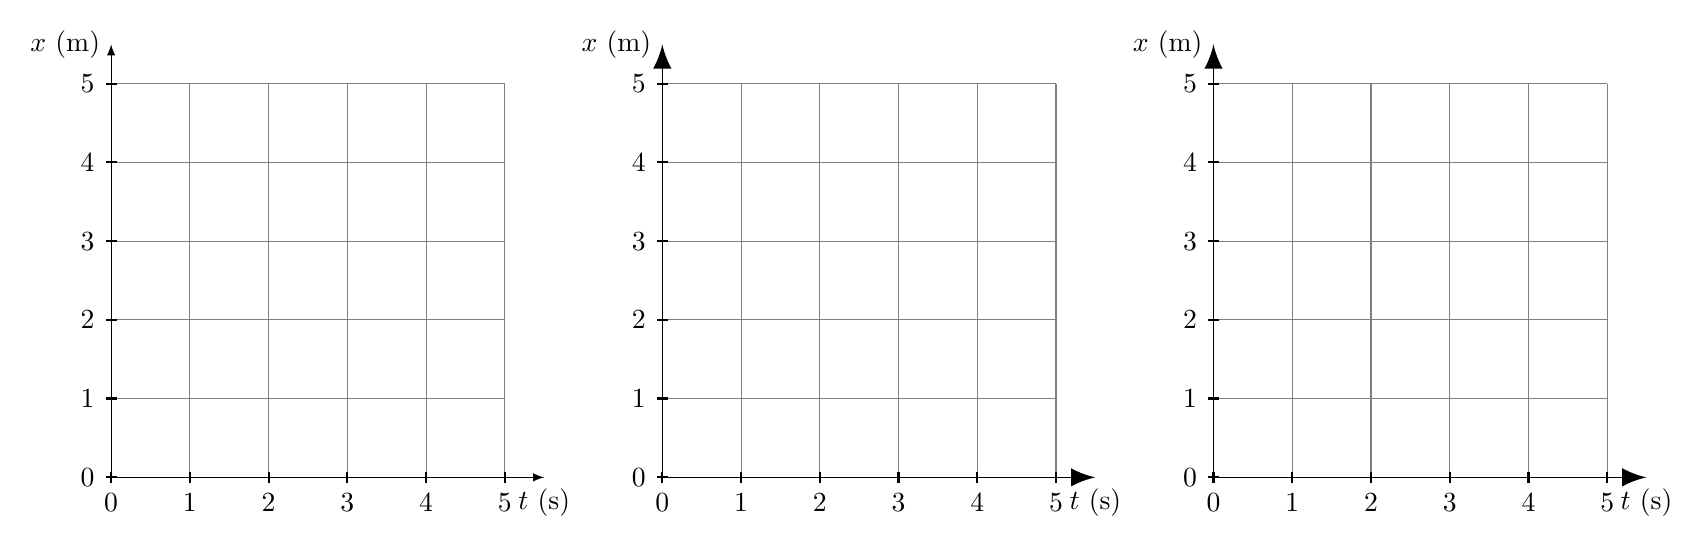
\begin{tikzpicture}
% Tableau en LaTeX standard avec tkz-text

% Repère quadrillé
\tkzInit[xmin=0,xmax=5,ymin=0,ymax=5, ystep=1]
\tkzGrid
\tkzDrawX[label = $t$ (s)]
\tkzDrawY[label = $x$ (m)]
\tkzLabelXY
\tkzFct[line width=2pt, domain=0:10]{2*\x}
\begin{scope}[xshift=7cm]
\tkzInit[xmin=0,xmax=5,ymin=0,ymax=5, ystep=1]
\tkzGrid
\tkzLabelXY

\tkzDrawX[label = $t$ (s)]
\tkzDrawY[label = $x$ (m)]
\tkzFct[line width=2pt, domain=0:10]{-2*\x+5}
\end{scope}
\begin{scope}[xshift=14cm]
\tkzInit[xmin=0,xmax=5,ymin=0,ymax=5, ystep=1]
\tkzGrid
\tkzLabelXY

\tkzDrawX[label = $t$ (s)]
\tkzDrawY[label = $x$ (m)]
\tkzFct[line width=2pt, domain=0:10]{2}
\end{scope}
\end{tikzpicture}

\end{document}
